%-------------------------------------------
\thispagestyle{empty}\cleardoublepage
\addcontentsline{toc}{section}{Keynote Talks}
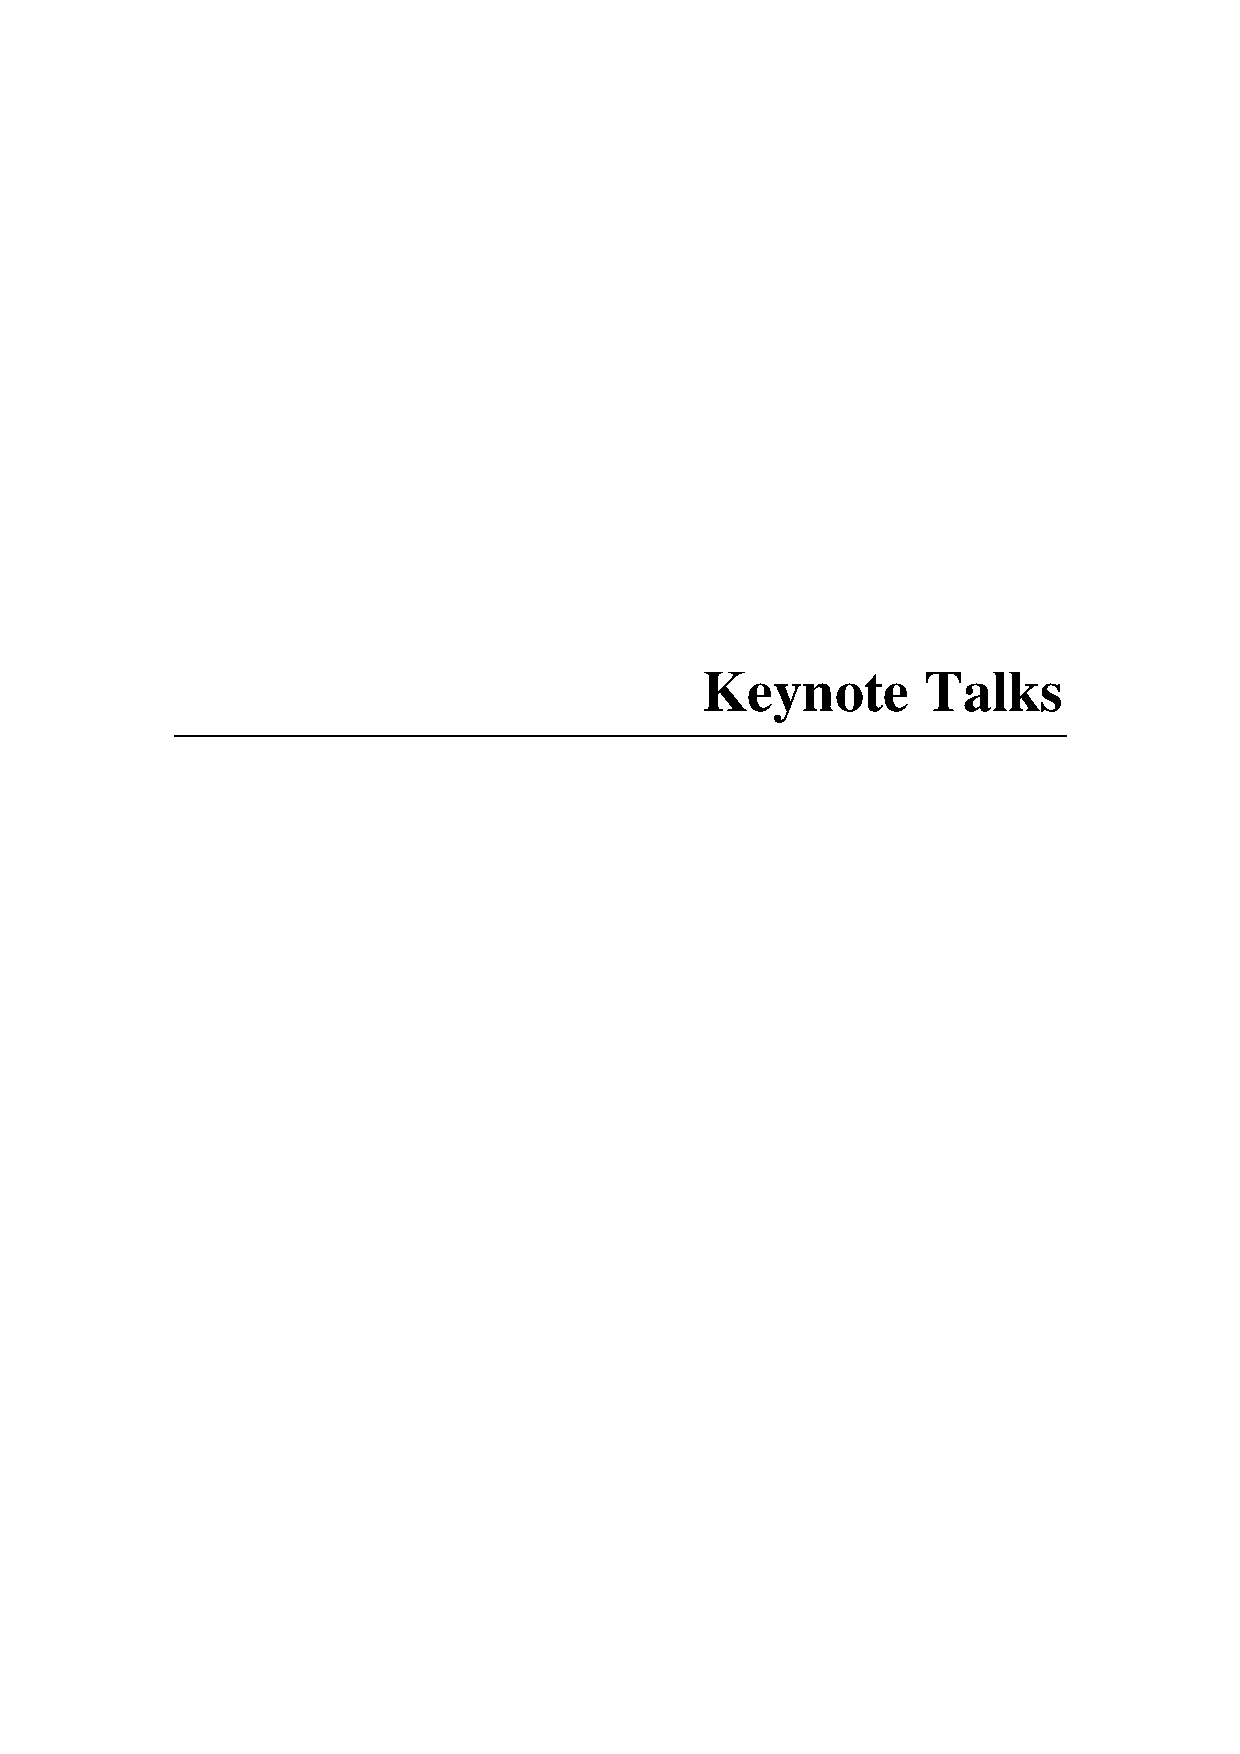
\includepdf[pages=1,pagecommand=\thispagestyle{empty}]{external/10_Keynotes.pdf}
\thispagestyle{empty}\cleardoublepage
 %-------------------------------------------
% Keynote talk 1
%\includeabstract{Keynote 1}{Speaker 1}{external/10-1_Keynotes-1.pdf}{}
\includeabstract{The New York Philharmonic Leon Levy Digital Archives:
An Integrated View of Performance Since 1842}{Barbara Haws, Archivist
and Historian, New York Philharmonic}{Abstract: For nearly 175 years the New York Philharmonic has been assiduously documenting and keeping all facets of its existence in whatever formats were available; marked conducting scores, orchestra parts, printed programs, business records, contracts, letters, newspaper reviews, audio and video. With the digitization of this material, it is possible for the first time to see the relationships between seemingly disparate materials that expand our understanding of the performance experience and the music itself. As well, especially through the GitHub repository, unanticipated applications of the data have occurred.   Working towards the year 2066, the challenge is to incorporate the new formats of the modern era to ensure that the single longest running dataset of a performing institution continues. 
}{Bio: Barbara Haws has been the Archivist and Historian of the New
York Philharmonic since 1984.  Haws has lectured extensively about the
Philharmonic’s past and curated major exhibitions here and in
Europe. She is a Grammy nominated producer of the Philharmonic’s
Special Editions historic recordings. Haws along with Burton Bernstein
is the author of Leonard Bernstein: American Original published by
Harper Collins, 2008 and the essay ``U.C. Hill, An American Musician
Abroad (1835-37)''. Since 2009, Haws has led an effort funded by the
Leon Levy Foundation to digitize more than three million pages of
archival material since 1842, making it freely available over the
internet. The Digital Archives project was recently featured on
FiveThirtyEight podcast ``What's The Point''.}

\thispagestyle{empty}\cleardoublepage
% Keynote talk 2
%\includeabstract{Keynote 2}{Speaker 2}{external/10-2_Keynotes-2.pdf}{}
\includeabstract{Is Machine Learning Enough?}{Beth Logan, PhD, VP, Optimization, DataXu}{Abstract: We live in a world unimaginable even 20 years ago.  From our phones we can summon a car, book a vacation and of course access the word’s music to find just those songs we like, even songs we didn't know we liked.  Automated Machine Learning at scale enables these and thousands more applications.   But in business, it’s good to know when to stop.  It's not always smart to automate that last, difficult 10\% of performance.  Indeed in music and other industries, humans often curate the results.  Will humans always be in the loop or will the machines eventually take over?   Will Machine Learning ever be enough?}{Bio: Beth is the VP of Optimization at DataXu, a leader in programatic marketing.  She has made contributions to a wide variety of fields, including speech recognition, music indexing and in-home activity monitoring.  Beth holds a PhD in speech recognition from the University of Cambridge.}
